\documentclass[a4paper,10pt]{article}


\usepackage[dvips]{graphicx}
\usepackage{amssymb,amsfonts,amsmath,color}
\usepackage{array}
\usepackage{graphicx}
\usepackage{caption}
\usepackage{amsmath}
\usepackage{graphics}
 %\usepackage{multirow}
 %\usepackage{sidecap}
%\usepackage[pdftex]{graphicx}
%\input{psfig.sty}
%\usepackage{wrapfig}
\usepackage{color}
\usepackage{graphicx}
\usepackage{caption}
\usepackage{url}
\usepackage{ragged2e} 
\usepackage{graphicx}
\usepackage{amssymb,color}
\usepackage{amsmath}
\usepackage{subfig}
\usepackage{array}
%\usepackage{sidecap}
\usepackage{amsmath}
\usepackage{wasysym}
\usepackage{amssymb,amsmath}
\usepackage{graphicx}
\addtolength{\oddsidemargin}{-.9in}
\addtolength{\evensidemargin}{-.9in}
\addtolength{\textwidth}{1.5in}
\addtolength{\topmargin}{-1.3in}
%\addtolength{\bottommargin}{-1in}
\addtolength{\textheight}{1.2in}
\def\CO2{CO$_2$}
\def\H2O{H$_2$O}
\def\3He{$^3$He}
\def\4He{$^4$He}
\def\CH4{CH$_4$}
\def\Kr{$^{84}$Kr}
\def\CH4{CH$_4$}
\def\RHe{$^3$He/$^4$He }
\def\wUS{western United States}
\def\degC{$^{\circ}$C }
\def\AR{$^{36}$Ar}
\def\Ar40{$^{40}$Ar}
\def\COHe{CO$_2$/$^3$He } 
\def\Ne{$^{20}$Ne}
\def\NeB{$^{21}$Ne}
\def\NeC{$^{22}$Ne}

\pagestyle{empty}
%opening

\title{Calculation of Deep Geothermal Gradient}

\author{Kiran Sathaye}

\begin{document}

\maketitle

\noindent The script \texttt{ODEHeat.py} calculates the the geothermal gradient below northeastern New Mexico. The heat produced by radioactivity in the crust is equal to the measured surface heat flux minus the input from the mantle

\begin{equation}
q_c=q_s-q_m = 58\frac{\text{mW}}{\text{m}^2}-28\frac{\text{mW}}{\text{m}^2}=30\frac{\text{mW}}{\text{m}^2}
\end{equation}

\noindent The upper crust is known to be more radioactive and less dense than the lower  crust, so the fraction of upper felsic crust is computed by using a seismic density profile from the USArray seismic network

\begin{equation}
f(z)=\frac{\rho(z)-3000}{2700-3000}.
\end{equation}

\noindent The mass fractions of the radioactive elements Uranium, Thorium, and Potassium can then be computed with depth,

\begin{eqnarray}
\text{U}(z)=f(z)\text{U}_{u}+(1-f(z))\text{U}_{l} \quad  \text{where} \quad  \text{U}_{l}=0.2\text{ ppm} \\
\text{Th}(z)=f(z)\text{Th}_{u}+(1-f(z))\text{Th}_{l} \quad  \text{where} \quad  \text{Th}_{l}=1.2\text{ ppm} \\
\text{K$_2$O}(z)=f(z)\text{(K$_2$O)}_{u}+(1-f(z))\text{(K$_2$O)}_{l} \quad \text{where} \quad   \text{(K$_2$O)}_{l}=0.6\%.
\end{eqnarray} 

\noindent Each radioactive isotope decays with a distinct energy, given by $E_{i}$, and at a known rate, $\lambda_i$.

\begin{eqnarray}
E_{238U}=7.4\cdot 10^{-12} \text{ J} \quad \lambda_{238U}=\frac{ln(2)}{4.468\cdot 10^9 \text{yr}} \\
E_{235U}=7.24\cdot 10^{-12} \text{ J} \quad \lambda_{235U}=\frac{ln(2)}{0.7038\cdot 10^9 \text{yr}} \\
E_{232Th}=6.24\cdot 10^{-12} \text{ J}  \quad \lambda_{232Th}=\frac{ln(2)}{14.05\cdot 10^9 \text{yr}} \\
E_{40K}=0.114\cdot 10^{-12} \text{ J}  \quad \lambda_{40K}=\frac{ln(2)}{1.248\cdot 10^9 \text{yr}}.
\end{eqnarray}

\noindent Combining the known total amount of heat production in the crust with the density profile gives the depth profile of radioactive elements and subsequent heat production with depth, 

\begin{eqnarray}
H_{238U}(z)=E_{238U}(6.022\cdot 10^{23})\lambda_{U238}\text{U(z)}\rho(z)/238 \quad  \text{W/m}^3\\
H_{235U}(z)=E_{235U}(6.022\cdot 10^{23})\lambda_{U235}\text{U(z)}\rho(z)/(235\cdot 137.88)  \quad \text{W/m}^3\\
H_{232Th}(z)=E_{232Th}(6.022\cdot 10^{23})\lambda_{Th232}\text{Th(z)}\rho(z)/232 \quad  \text{W/m}^3\\
H_{40K}(z)=2(120\cdot 10^{-6})E_{40K}(6.022\cdot 10^{23})\lambda_{K}\text{K$_2$O}(z)\rho(z)/94 \quad  \text{W/m}^3
\end{eqnarray}

\noindent Thermal conductivity of the crust varies inversely with temperature, 

\begin{eqnarray}
k_{fels}(T)=1.64+\frac{807}{350+T(^{\circ}\text{C)}} \frac{W}{mK^{\circ}} \quad \text{and} \quad k_{maf}=2.18+\frac{474}{350+T(^{\circ}\text{C)}}  \frac{W}{mK^{\circ}}.
\end{eqnarray}

\noindent Because conductivity and temperature are co-dependent, and the heat flux and temperature are known at the surface, the temperature is solved for iteratively moving down into the crust, 
\begin{equation}
\frac{dq}{dz}=-H(z) 
\end{equation}

\begin{equation}
k_s\Big(\frac{dT}{dz}\Big)_{s}=-q_s.
\end{equation}

\noindent Written in a finite difference form, the solution for temperature is 

\begin{equation}
T_{i+1}=T_i-\frac{q_i(\rho_i,f_i)dz_i}{k_i(f_i,T_i)}.
\end{equation}


\section{Inverse Problem}

\subsection{Mineralogy}

\noindent We first define an indicator function $w_i$ to indicate the mixture of mineralogies in the crust and shallow mantle.  This is a piecewise function determined by the rock density $\rho$, defined as 

  \[
    w_{water} = \left\{\begin{array}{rr}
        (2.7-\rho)/(2.7-1), & \text{for } 1\leq \rho  \leq  2.7\\
        0, & \text{for } 2.7 \leq \rho \\
        \end{array}\right\} 
  \]

  \[
    w_{fels} = \left\{\begin{array}{rr}
        0, & \rho \leq 1 \\
    	(\rho-1)/(2.7-1), & \text{for } 1 \leq \rho \leq2.7\\\
	(3-\rho)/(3-2.7), & \text{for } 2.7\leq \rho  \leq  3\\
        0, & \text{for } 3 \leq \rho \\
        \end{array}\right\} 
  \]
  
    \[
    w_{maf} = \left\{\begin{array}{rr}
    	0, &  \text{for }  \rho  \leq  2.7\\
        (\rho-2.7)/(3-2.7), & \text{for } 2.7\leq \rho  \leq  3\\
        (3.3-\rho)/(3.3-3), & \text{for } 3\leq \rho  \leq  3.3\\
        0, & \text{for } 3 \leq \rho \\
        \end{array}\right\} 
  \]
  
      \[
    w_{mantle} = \left\{\begin{array}{rr}
    	0, &  \text{for }  \rho  \leq  3\\
        (3-\rho)/(3.3-3), & \text{for } 3\leq \rho  \leq  3.3\\
        1, & \text{for } 3.3 \leq \rho \\
        \end{array}\right\}
  \]
 
       \[
    \sum_{i=1}^4 w_i =1.
  \]
  \subsection{Conductivity}
  
  \noindent Thermal conductivity of minerals varies inversely with temperature. The  conductivity [W/m/$^{\circ}$C] for mineral $i$ at a temperature given in $^{\circ}$C, is 
  
  \begin{equation}
  k_i=A_i+\frac{B_i}{350+T}.
  \end{equation}
  
  \noindent The coefficients $A_i$ and $B_i$ have been estimated through experiment, but need to be tuned to the temperature measurements at the surface and estimates at the mantle.  
  
  \subsection{Heat Conduction Equation}
  
  Using previously defined values for $w_i$ and $k_i$, the steady state heat conduction equation through the Earth's crust and shallow mantle becomes
  
  \begin{equation}
  \frac{d}{dz} \left(\sum_{i=1}^4\left(A_i+\frac{B_i}{350+T}\right)w_i\frac{dT}{dz}\right)=\sum_{i=1}^4w_iH_i.
  \end{equation} 
  
 \noindent This equation can be constrained using boundary conditions for the temperature at the surface and at 70km depth, 
 
 \begin{equation}
 T \Big |_{z=0}=T_S \quad \mbox{and} \quad T \Big |_{z=70km}=T_{m}.
 \end{equation}
 
 \noindent The inverse problem is then solved my minimizing the error in the heat production and conductivity variables using measurements of surface heat flux and estimates of heat flux from the crust into the mantle. The largest component of the cost function is terms to minimize the error between the modeled and observed heat flux at the surface and at the bottom of the crust.  The flux constraints in the cost function are 
 
 \begin{equation}
C_1=\frac{1}{2} \left| q_s-k(0)\frac{dT}{dz}\Big|_{z=0} \right |^2 \quad \mbox{and} \quad C_2=   \frac{1}{2} \left| q_m-k(70km)\frac{dT}{dz}\Big|_{z=70km} \right |^2.
 \end{equation}
 
 \noindent There are empirical estimates of the conductivity coefficients $A_i$ and $B_i$, as well as crustal heat production $H_i$. Therefore, the computed value can be compared to the empirical values. These values are subject to much higher uncertainty and are therefore weighted much lower according to their variances $\alpha_i, \beta_i, \text{and } \eta_i$.  

 \begin{equation}
C_3=\sum_{i=1}^3\frac{\alpha_i}{2}\left | A_i-A^{pr}_i\right |^2 \quad \quad  C_4=\sum_{i=1}^3\frac{\beta_i}{2}\left | B_i-B^{pr}_i\right |^2 \quad  \quad C_5=\sum_{i=1}^3\frac{\eta_i}{2}\left | H_i-H^{pr}_i\right |^2.
 \end{equation}
 
 
\noindent The solver will then iterate until minimizing the cost function over the 11 variables shown above, 
 
 \begin{equation}
 min \sum_{i=1}^5 C_i.
 \end{equation}
 
\subsection{Temperature Constraints}
  
Boundary conditions can be placed on temperature by using observed mean annual surface temperature and estimates base on S-Wave speeds at a depth of 70km.  
  
\begin{figure}[h]
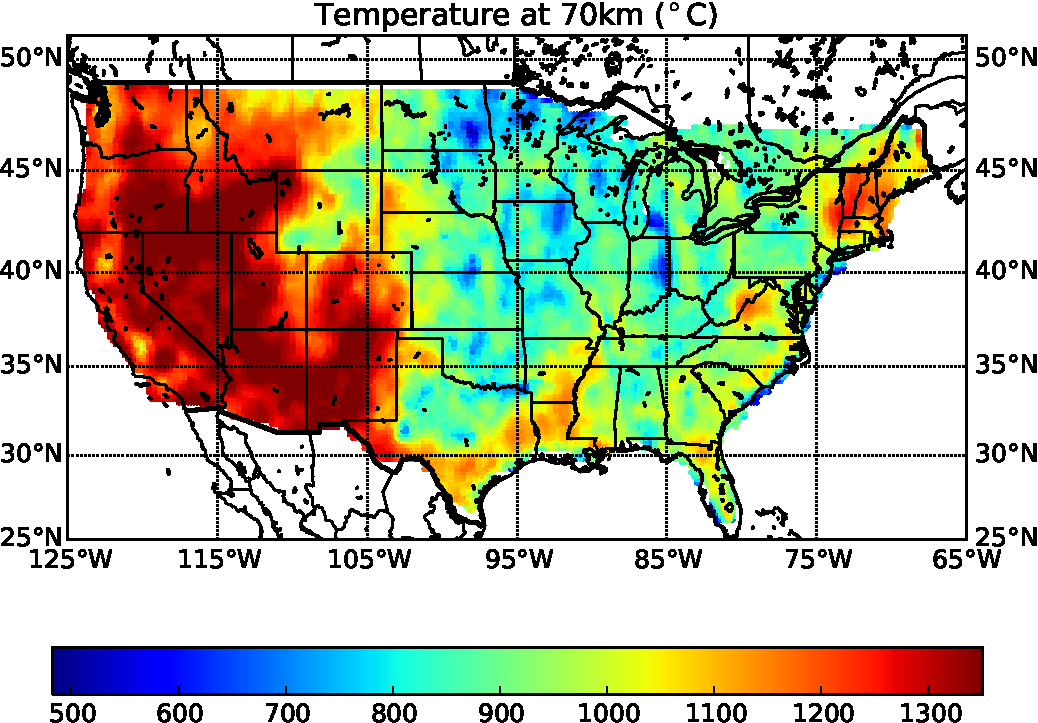
\includegraphics[width=0.49\textwidth]{TempMap70-crop.pdf} \quad
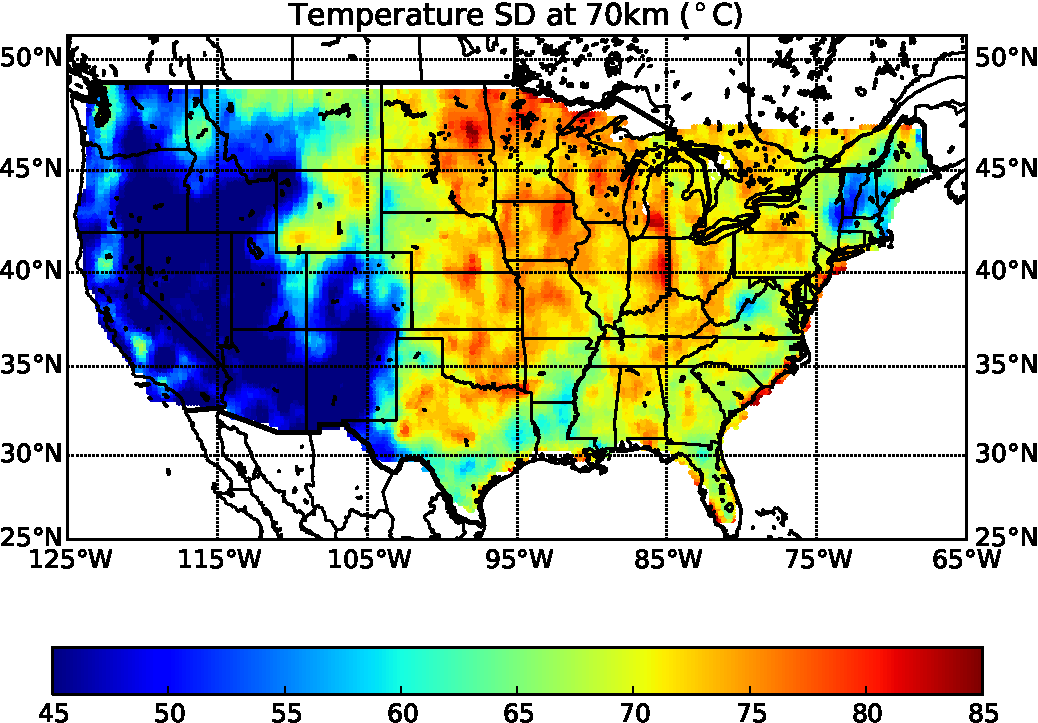
\includegraphics[width=0.49\textwidth]{UncertainTempMap70-crop.pdf}
\caption{Temperature and associated uncertainty at 70km depth.}
\end{figure}
  
  
\subsection{Conductivity Constraints}
  
Thermal conductivities for various mineralogies have been measured and used to determine  temperature dependence.  However, these coefficients give erroneously low conductivity values, causing geothermal gradients to be computed much higher than can be reasonably expected. However, these listed coefficients can be used as a guide in the cost function minimization, ensuring $A_i$ and $B_i$ with reasonable values. The thermal conductivity of water has a slight positive correlation with temeprature, varying between 0.6 and 0.7 (W/m/$^{\circ}$C) in subsurface conditions.   \\
  
\centering
\label{my-label}
\begin{tabular}{lllll}
            & A   (W/m/$^{\circ}$C)   & B  (W/m)   & Range  ($^{\circ}$C) &  \\
Salt        & -2.11 & 2960 & -20  to  40\\
Limestone   & 0.13  & 1073 & 0   to 500 \\
Metamorphic & 0.75  & 705  & 0 to 1200 \\
Felsic      & 0.64  & 807  & 0   to 1400 \\
Mafic       & 1.18  & 474  & 50 to 1100 \\
Ultra Mafic & 0.73  & 1293 & 20 to 1400           
\end{tabular}
  \justify
  
 The solutions with listed conductivity values give unrealistically high geothermal gradients, leading to large overestimates of the temperature at 70km depth. Therefore, reasonable thermal conductivities will have to be computed using the inverse method discussed above. 
 
 
 \begin{figure}
 \centering
 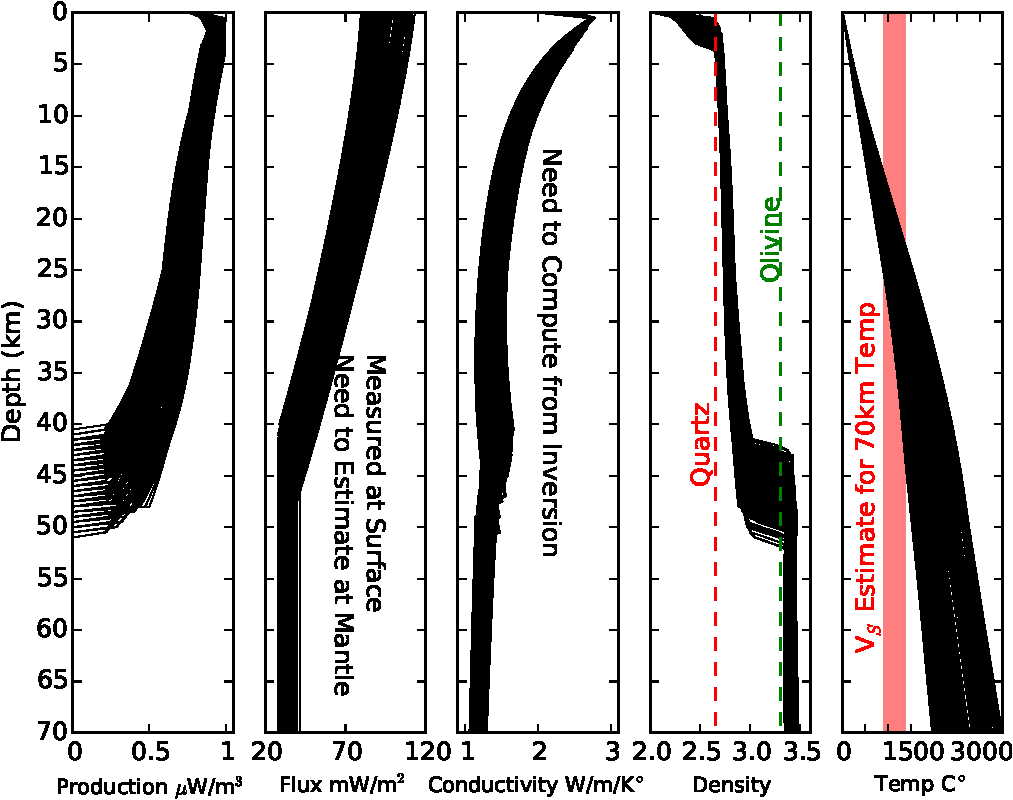
\includegraphics[width=.45\textwidth]{HeatFluxProd-crop.pdf} 
  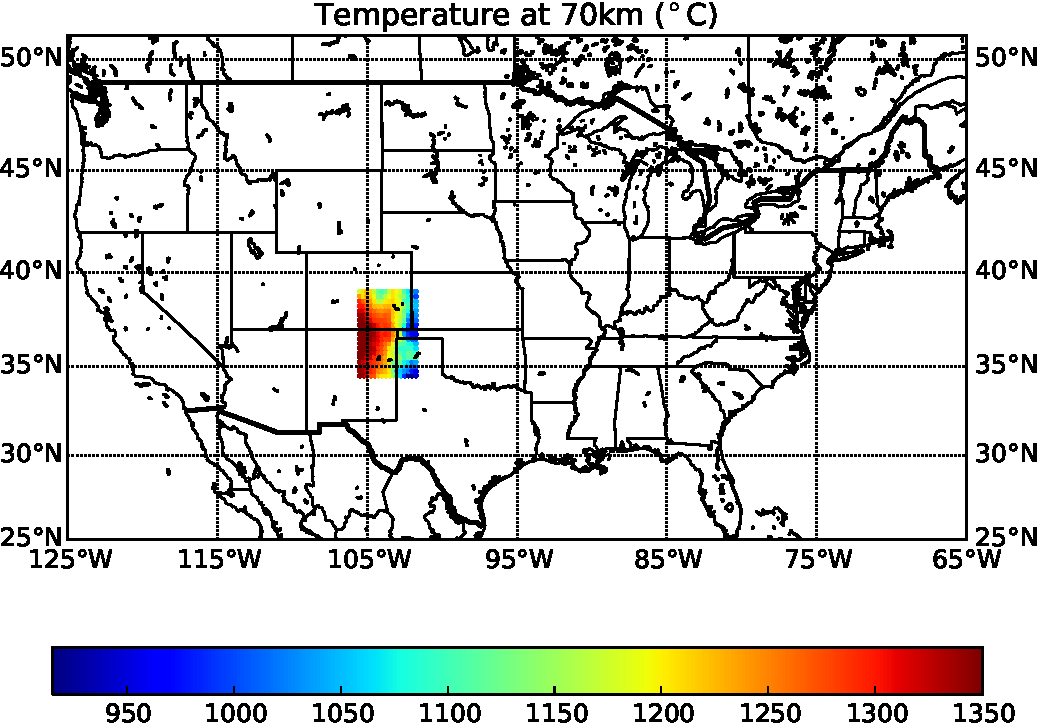
\includegraphics[width=.52\textwidth]{Temp70Seismic-crop.pdf} 
 \caption{Geothermal gradients computed in northeastern New Mexico using listed thermal conductivity and mantle flux values for 304 seismic profiles. Estimates are much higher than reasonable values from S-wave inversion.  }
 \end{figure}
\subsection{Heat Production Constraints} 
  
 Heat production constraints are derived from geochemical estimates of the main radioactive elements in the Earth's crust, uranium, thorium and potassium  (Rudnick and Fountain, Reviews of Geophysics 1995). These elements are enriched in the crust relative the mantle, and in the upper crust relative to the lower crust. However, these compositions greatly overestimate the overall heat production from the Earth's crust, leading to a large discrepancy with observed heat fluxes at the surface.  Therefore, these listed compositions will be used as a guide in the cost function minimization, not as a hard constraint.   \\
 
\centering
\label{my-label}
\begin{tabular}{lllll}
             & Uranium & Thorium & K$_2$O (\%) & Heat Production  \\
Upper Crust  & 2.8ppm           & 10.7ppm          & 3.4(\%)          & 1.65($\mu$W/m$^3$)\\
Middle Crust & 1.6ppm           & 6.1ppm           & 2.01(\%)         & 1.00($\mu$W/m$^3$) \\
Lower Crust  & 0.2ppm           & 1.2ppm           & 0.6(\%)          & 0.19($\mu$W/m$^3$)                          
\end{tabular}
 
\subsection{Flux Constraints}
 
 \justify
 
Heat fluxes have been measured at the Earth's surface by the SMU Geothermal Lab, and estimated at the crust-mantle boundary by (Artemieva and Mooney JGR 2001).  These fluxes will be used to compute the objective function  of the heat conduction equation.  
  
\begin{figure}[h]
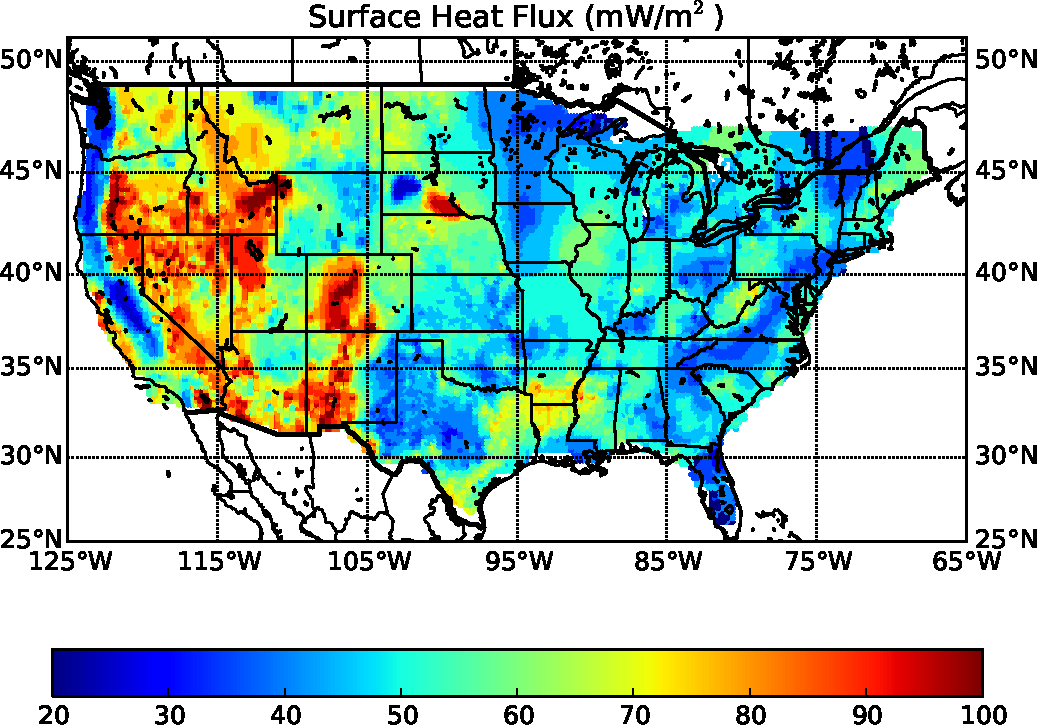
\includegraphics[width=0.49\textwidth]{HeatMapUSAr-crop.pdf} \quad
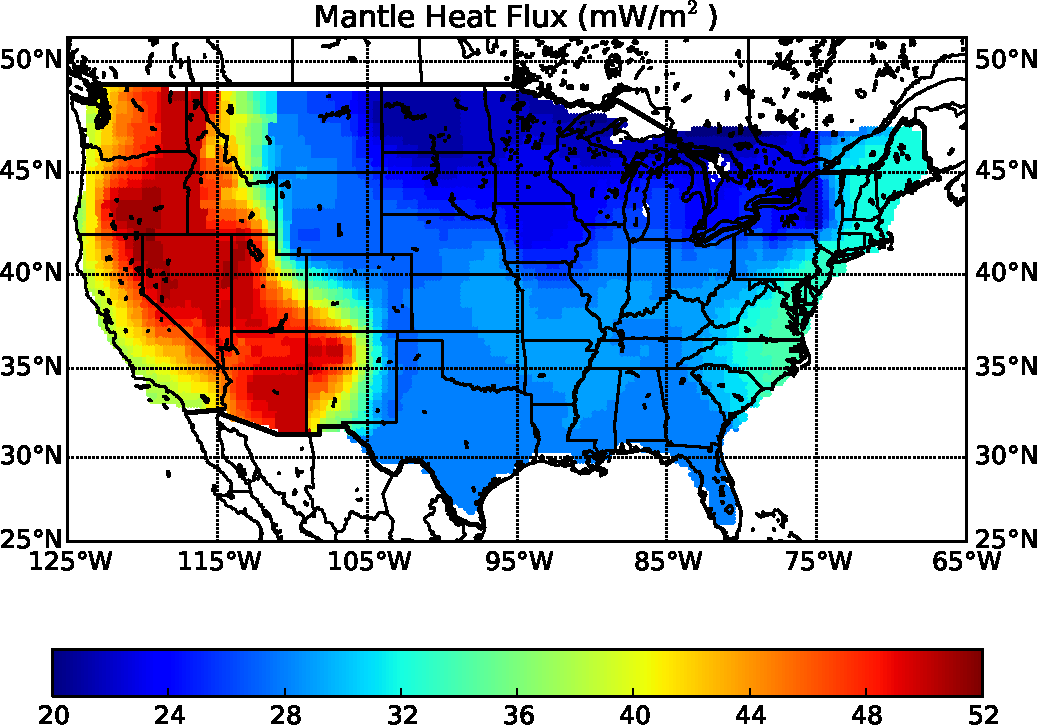
\includegraphics[width=0.49\textwidth]{MantleFlux-crop.pdf}
\caption{Flux estimates at the surface and mantle-crust boundary.  Surface heat flux will be used as a hard constraint for optimization, while mantle heat flux will be treated as a less weighted constraint.}
\end{figure}
  
\end{document}

